\section{B-alberi}

I B-alberi sono \textbf{alberi bilanciati} adatti per memorizzare grandi masse di dati in memoria secondaria. Sono simili agli alberi rosso-neri, ma sono progettati per minimizzare gli accessi alla memoria secondaria. Le operazioni sono \textbf{insert}, \textbf{delete}, \textbf{search}, \textbf{split} e \textbf{join}.

I nodi dei B-alberi possono avere un numero di chiavi $n\ge 1$ ed $n+1$ figli.

\begin{figure}[htpd]
\centering
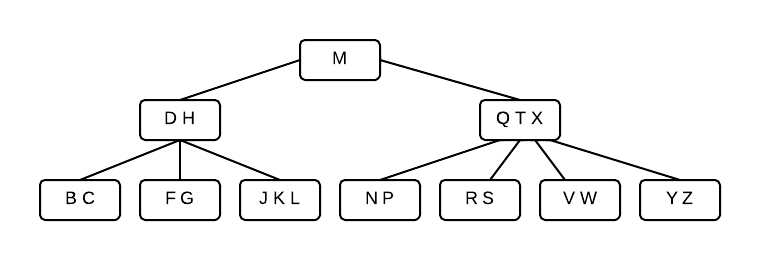
\includegraphics[width=100mm]{images/b-alberi1.png}
\end{figure}

\subsection{Definizione di un B-albero}

Un B-albero $T$ è un albero di radice $T.root$ tale che:

\begin{enumerate}

\item Ogni nodo $x$ contiene i seguenti campi:
	\begin{enumerate}
	\item $x.n$: il numero di chiavi presenti nel nodo;
	\item $x.key_1\le x.key_2 \le ... \le x.key_n $: le $x.n$ chiavi in ordine crescente;
	\item $x.leaf$: valore booleano che è true se il nodo $x$ è una foglia, false altrimenti.
	\end{enumerate}
\item Se il nodo non è una foglia contiene anche $x.c_1, X.c_2, x.c_{n+1}$: gli $n+1$ puntatori ai figli;
\item Le chiavi $x.key_1, x.key_2, ..., x.key_n$ di un nodo interno separano le chiavi dei sottoalberi. Se $k_i$ è una chiave qualsiasi del sottoalbero $x.c_i$, allora:

$$k_1 \le x.key_1 \le k_2 \le x.key_2 \le ... \le x.key_{x.n} \le k_{x.n+1}$$

\item Le foglie sono tutte alla stessa profondità $h$, detta \textbf{altezza dell'albero};
\item Vi sono limiti inferiori e superiori al numero di chiavi in un nodo, e tali limiti dipendono da una costante $t$ detta \textbf{grado minimo} del B-albero.
	\begin{enumerate}
	\item Ogni nodo, eccetto la radice, ha almeno $t-1$ chiavi e, se non è una foglia, ha almeno $t$ figli;
	\item Se l'albero non è vuoto la radice contiene almeno una chiave;
	\item Ogni nodo ha al più $2t-1$ chiavi e, se non è foglia, ha al più $2t$ figli.
	\end{enumerate}

\end{enumerate}

Ad ogni chiave sono generalmente associate delle informazioni ausiliarie. Assumeremo implicitamente che quando viene copiata una chiave vengono copiate anche tali informazioni. I B-alberi più semplici sono quelli con grado minimo $t=2$. Ogni nodo interno ha 2,3 o 4 figli.
Ogni albero non vuoto di grado minimo $t$ con $N$ chiavi ha altezza:

$$h \le \log_t\frac{N+1}{2}$$

\subsection{Operazioni sui B-alberi}

Adottiamo le seguenti convenzioni per le operazioni sui B-alberi:

\begin{enumerate}

\item La radice del B-albero è sempre in memoria;
\item I nodi passati come parametri alle procedure sono stati preventivamente caricati in memoria.

\end{enumerate}

\subsubsection{Creazione di un B-albero vuoto}

La procedura ausiliaria \textbf{ALLOCATE-NODE} alloca una pagina del disco da utilizzare come nuovo nodo nel tempo $O(1)$. Supponiamo che un nodo creato da ALLOCATE-NODE non richieda l'operazione DISK-WRITE.

\begin{lstlisting}[caption=Creazione di un B-albero]

B-TREE-CREATE(T)
	x = ALLOCATE-NODE()
	x.leaf = true
	x.n = 0
	DISK-WRITE(x)
	T.root = x

\end{lstlisting}

La procedura B-TREE-CREATE richiede $O(1)$ operazioni su disco e quindi un tempo di CPU pari a $O(1)$.